\providecommand{\main}{../../..}
\providecommand{\Figures}{\main/Figures}

\documentclass[\main/main.tex]{subfiles}

\begin{document}
                    
\section{Vers un recalage plus robuste et des segmentations plus précises et versatiles}

%
Dans leurs états actuels, les algorithmes de segmentation, relativement lents, permettent d'obtenir des résultats robustes. En revanche, les algorithmes de recalage présentent des failles prévisibles possibles à corriger dans le futur.
Je présente ci-dessous des pistes pour améliorer les segmentations et le recalage,
ainsi que des solutions pour réduire les temps de calculs nécessaires.

    \subsection{L'étude de la symétrie du cerveau permettrait d'améliorer la qualité du recalage}
 
%   
La méthode de recalage actuellement développée est basée sur la segmentation automatique des cristallins ainsi que sur une segmentation grossière de la matière blanche. Cet algorithme possède un certain nombre de défauts, principalement liés à l'utilisation des cristallins, qui malheureusement ne sont pas détectables dans toutes les souches de \pz{}, en particulier celles qui possèdent des mutations de pigmentation .
%
Avec plusieurs mutations de pigmentation, la souche de \pz{} casper présente une forte dépigmentation sur tout le corps~\cite{white_2008}, qui la rend très utile en imagerie du \pz~\cite{hecker_2020,camiolo_2020, wertman_2020}, en permettant d'étudier les patrons de protéines fluorescentes natives. Lors de la clarification des échantillons, elle permet ainsi d'éviter  l'étape de dépigmentation, qui dénature les protéines fluorescentes, et rend  nécessaires les longs protocoles utilisant des anticorps.   Néanmoins, chez les casper, la rétine reste pigmentée, ce qui rend impossible la pénétration de la lumière dans l'oeil et donc l'observation du cristallin, indispensable au recalage
%%
%
Il est possible d'adapter l'algorithme de segmentation du cristallin à la segmentation de l'oeil pour définir un axe de référence permettant le recalage. En effet, l'oeil est recouvert par une structure marquée par les marqueurs lipophiles, au moins dans la partie supérieure. Ainsi, dans une image 3D obtenue avec un microscope confocal, l'oeil prend la forme d'une demie sphère possèdant des valeurs de gris nulles. En diminuant le coefficient de sphéricité utilisé  pour reconnaître les cristallins, l'algorithme va identifier l'oeil comme le plus grand objet quasi-sphérique et obscur au sein de l'EE.
Ainsi, l'axe inter-oculaire est identifié comme axe de référence. Néanmoins, comme l'oeil est plus grand que le cristallin, il est possible que les échantillons soient moins précisément recalés.
%%
%
Une seconde possibilité consiste à identifier un plan de symétrie permettant de définir un premier axe de référence.
%
Comme le cerveau est symétrique par rapport au plan sagittal, il devrait être aussi possible d'utiliser le vecteur normal au plan de symétrie de le segmentation de la matière blanche comme axe de référence. Ainsi ,le recalage ne se baserait que sur la segmentation de la matière blanche.
%
De nombreuses publications décrivent des algorithmes de détection automatique du plan de symétrie du cerveau, en particulier dans des images acquises par imagerie par résonance magnétique ou par scanner ~\cite{tan_2019,noori_2020,rehman_2018}. En adaptant ces méthodes publiées au \pz{}, on obtiendrait sans douite un algortithme ayant une robustesse supérieure.
%
Cependant, la segmentation de la matière blanche est actuellement effectuée  rapidement, et les axes obtenus par la détection de l'ellipsoïde entourant une segmentation approximative de la matière blanche pourrait induire une certaine imprécision. Une procédure de segmentation plus précise serait donc peut-être nécessaire, mais son trop long temps de calcul est actuellement incompatible avec un traitement des échantillons suffisamment rapide pour traiter de nombreux échantillons dans le cadre du \hcs{}.
Il est donc nécessaire de développer de nouvelles stratégies de segmentations plus rapides.

    \subsection{Vers des segmentations plus rapides et plus précises avec l'apprentissage profond}

%    
Dans le cadre de ce projet, quatre méthodes de segmentations ont été développées et validées: la segmentation de l'ensemble de l'échantillon, de la matière blanche, de la matière grise, et des cristallins.
%
Cependant, ces segmentations sont actuellement lentes, avec une durée de deux à six minutes.

Je présente une stratégie qui pourrait permettre d'accélérer les calculs tout en obtenant des résultats précis.
%%
%
Durant la dernière décennie, les algorithmes d'apprentissage profond ont permis la développement d'outils pour la segmentation automatique de tout type d'organes acquis par divers systèmes d'imagerie~\cite{gottapu_2018,oztel_2017,zhang_2020,hossain_2019}~\cite{long_2015,ronneberger_2015,Milletari_2016}.
%
Ces méthodologies ont été développé car elles sont robustes et rapides une fois entraînées. Elles peuvent de plus être couplées à des annotations manuelles et l'utilisation de plusieurs annotations sur le même jeu d'entraînement permet de générer une segmentation par région d'intérêt~\cite{zhao_2019,tong_2018,feng_2019}.
%
La multiplication des calculs nécessaires pour obtenir les résultats de segmentation rendent nécessaire l'utilisation de coûteuses cartes graphiques dédiées.
%
De plus, cette méthode nécessite une étape d'entraînement du réseau de neurones qui peut être lourde ~\cite{ghafoorian_2017,jiang_2018,xu_2018}.
%
Cette étape nécessite en effet de recalculer un grand nombre de fois les différents poids du réseau de neurones. De plus, cette étape d'entraînement nécessite des jeux d'images annotées manuellement pour indiquer les régions à segmenter. 
%
Les nombre d'images nécessaires pour cette étape est proportionnel à la profondeur du réseau de neurones, et parfois, en raison de la rareté de l'échantillon à étudier, ou bien de la complexité de la structure d'intérêt, il peut être impossible d'obtenir suffisamment d'images de référence. Des solutions doivent alors être trouvées, soit pour simplifier l'annotation, soit pour réduire le nombre d'images pour l'entraînement.
%
Pour simplifier l'annotation, des procédures de segmentations préliminaires rapides ont été développées~\cite{rajchl_2017}. Elles rendent possible le calcul rapide de segmentations précises des régions d'intérêt identifiées qui pourront alors être utilisées comme images de référence pour de futurs segmentations.
%
Une autre possibilité  d'effectuer de l'apprentissage par transfert en utilisant des réseaux de neurones pré-entraînés à réaliser des segmentations automatiques différentes des segmentations désirées.

L'emploi d'une méthode d'apprentissage par réseau de neurones profonds couplé à un apprentissage par transfert pourrait ainsi permettre d'améliorer la précision de la segmentation tout en réduisant le temps de calcul nécessaire à sa réalisation.

    \subsection{La segmentation d'autres régions d'intéret permettrait d'augmenter la versatilité de la plateforme ZBI}
 
%   
Les segmentations que j'ai développé au cours de ma thèse visent à automatiser la mesure du cerveau.
%
Cependant, comme le montre l'exemple de la segmentation du cristallin,
il est possible de détecter d'autres organes grâce aux marquages employés.
%
De plus, comme vu en section~\ref{sec:marqueurs}, le développement de nouveaux marqueurs nécessitera la mise en place de nouveaux algorithmes adaptés aux objets à détecter.
%
Je vais maintenant donner des exemples segmentations pouvant être réalisées, ainsi que les algorithmes à développer pour automatiser ces segmentations.

%
Le marqueur lipophile permet de mettre en évidence les lipides, et donc l'ensemble des membranes cellulaires. De plus, l'absence de marquage au sein d'une région peut aussi permettre de les segmenter.
%
En utilisant cette propriété, deux autres types de tissus paraissent identifiables en utilisant l'absence de marquage. La notochorde est une structure tubulaire située sous le tube neural\ref{fig:notochord}. Elle joue le rôle de squelette pour les embryons.

\ajout{
\begin{figure}[!h]
    \centering
    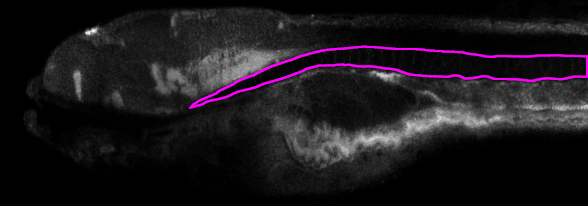
\includegraphics[width = \textwidth]{\Figures/discussion_info/notochord_seg.png}
    \caption{
    Coupe parasagittale d'une acquisition confocale d'un marquage lipophile d'un alevin de \pz{}.
    \newline
    La notochorde est une structure tubulaire servant de squelette aux alevins.
    La notochorde étant une structure faiblement marquée par le marqueur lipophile, la segmentation de cette région pourrait être réalisée par la recherche de la plus longue région tubulaire ayant de faibles valeurs de gris.
    \newline
    La ligne magenta représente la délimitation de la segmentation manuelle de la notochorde.
    }
    \label{fig:notochord}
\end{figure}
}

Avec un marqueur lipophile, elle est reconnaissable car il s'agit d'une région de très faible intensité lumineuse. Ainsi, une fois l'EE segmenté,
la détection de la notochorde pourrait être réalisée en cherchant une région cylindrique de très faible intensité.
%
Au vue de la simplicité de la forme à détecter, cette détection pourrait être effectuée en suivant les étapes suivantes: d'abord, la segmentation de la larve entière, puis un seuillage manuel en prenant une valeur très basse de gris, ensuite une fermeture par segment qui conserve uniquement les éléments linéaires, et finalement la sélection du plus grand objet, en l'occurence la notochorde.
D'autres structures d'intérêt ne présentant pas de marquage sont les deux vésicules otiques, sous-partie de l'oreille interne des vertébrés. Elles se trouvent entre la peau et le médula oblongata, et sont symétriques par rapport au plan sagittal du cerveau.

%
Avec un marqueur lipophile, les otolithes constituent deux régions ovoïdes à faibles valeurs de gris, qui peuvent être segmentées selon le protocole suivant.
Une fois les segmentation de la larve entière et de la matière blanche obtenues, on recherche l'axe de symétrie de la matière blanche au sein de la larve. On effectue ensuite un seuillage au sein de la larve afin de détecter les régions ayant des valeurs de gris très faibles. En utilisant la position de la matière blanche, on recherche alors deux éléments placés symétriquement par rapport au cerveau et se trouvant proche de la limite interne de la segmentation. Ainsi, cette information permet de faire la distinction avec les deux yeux (en fond casper).

\ajout{
\begin{figure}[!h]
    \centering
    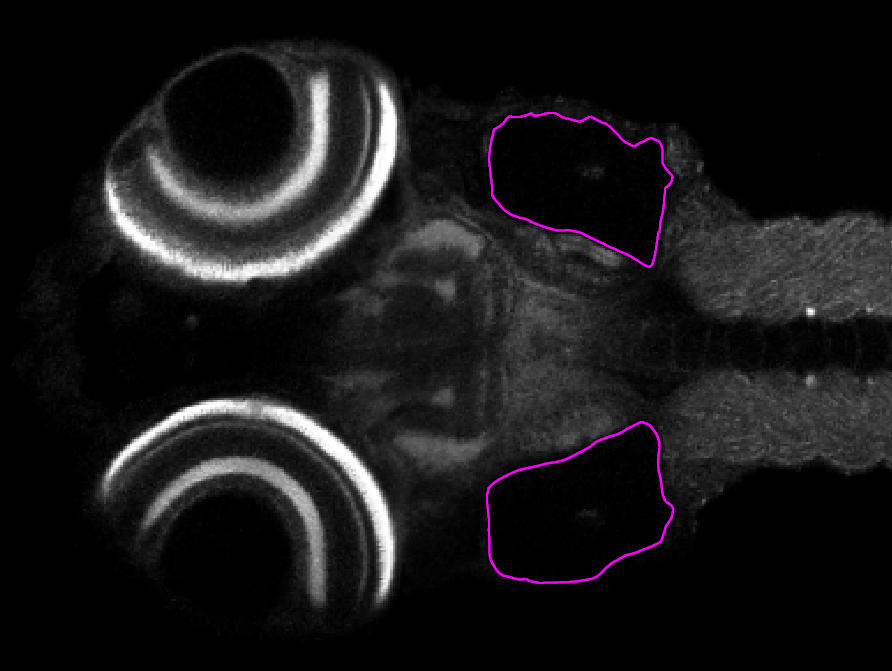
\includegraphics[width = \textwidth]{\Figures/discussion_info/otic_vesicul_seg.png}
    \caption{
    Coupe transversale d'une acquisition confocale d'un marquage lipophile d'un alevin de \pz{}.
    \newline
    Les vésicules otiques sont deux structures situées symétriquement par rapport à l'axe parasagittal de l'alevin, entre la peau et la médula oblongata.
    S'agissant de régions faiblement marquées par le marqueur lipophile, leurs segmentations pourraient être réalisées en s'appuyant sur la segmentation de la matière blanche.
    \newline
    Les lignes magentas représente les délimitations de segmentations manuelles des vésicules otiques.
    }
    \label{fig:notochord}
\end{figure}
}

%%
%
La détection d'autres tissus peut être réalisée avec d'autres marquages. Comme dernier exemple, je vais présenter la segmentation du réseau vasculaire.
Au chapitre~\ref{chap:bio:marqueurs:vasc}, j'ai expliqué qu'un marquage présent dans une lignée Kdrl-RFP marque le système vasculaire du \pz{}.
%
La segmentation automatique de structures curvilignes comme les vaisseaux est complexe et constitue un sujet de recherche à part entière. Trois stratégies différentes permettant de réaliser de telles segmentations.

%%
%
Afin d'obtenir rapidement un résultat de segmentation, il est possible d'employer un seuillage automatisé~\cite{kugler_2019}, approche simple à mettre en place.
%
Cependant, comme nous avons pu le voir précédemment, cette méthode particulièrement sensible au bruit et à l'homogénéité de l'histogramme des valeurs de gris de l'image. Il est donc préférable d'utiliser d'autres approches plus robustes. Une fermeture morphologique peut par exemple être effectuée en utilisant comme élément structurant un ensemble de lignes à orientations variées, qui permettent de détecter des structures linéaires~\cite{Soille_2001}. Ces approches ne sont pas néanmoins pas très efficaces pour la détection de structures sinueuses, ce qui les rend peu adaptées à la détection du système vasculaire.
%
Des méthodes de fermetures par chemins ont été développées~\cite{talbot_2007,merveille_2018}. Ces chemins permettent ainsi de suivre les sinuosités de structures curvilignes, ce qui permet de réaliser la segmentation de vaisseaux sanguins. Cette stratégie présente une forte robustesse en cas d'image non homogène ou bruitée.
%
L'emploi d'un réseau de neurones profonds pour la segmentation automatique de vaisseau de \pz{} a déjà été effectuée dans d'autres cadres ~\cite{zhang_2019a, daetwyler_2019}.
%
Comme vu précédemment, il est possible de simplement utiliser un transfert de réseau de neurones afin de permettre de diminuer le quantité de données nécessaires à l'entraînement du réseau de neurones. Ces segmentations pourraient donc servir de base au développement de méthode chez le \pz{}.


\end{document}
